\section{Motor med tilh. H-bro på bil}

Motorkredsløbet for AU2 vil potentielt være et større EMC-problem, da en højfrekvent og stor strøm løber igennem dele af kredsløbet. Selve motoren vil producere en stor støj, og for at modvirke dette er der placeret en kondensator parallelt med motoren, som derved fjerner en stor del højfrekvent støj som opstår da motoren er en induktiv belastning. 

\begin{figure}[h]
\centering
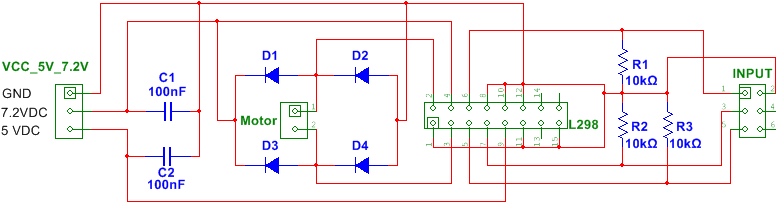
\includegraphics[width=\textwidth]{../fig/billeder/hbro_multisim.png}
\caption{Design af motorens Hbro i Multisim.}
\label{fig:hbro_multisim}
\end{figure}

Motoren har nogle strømloop, som hhv. kan løbe den ene og den anden vej, når hbroen skifter retningen af DC-motoren. Dog vil det kun have betydning for ledningerne før motoren, da transistorerne er konstant tændte/slukkede i parvis. Denne måde at bruge kredsløbet sikrer at vi ved hjælp af kondensatoren som er parallel med motoren, kan lempe støjen en del. Dog vil strømmen der tænder og slukker i ledningerne før motoren, kunne give problemer ifm. nærværende ledninger/printbaner. 
Strømloops kan ses på figur \ref{fig:hbro_multisim_loop}

\begin{figure}[h]
\centering
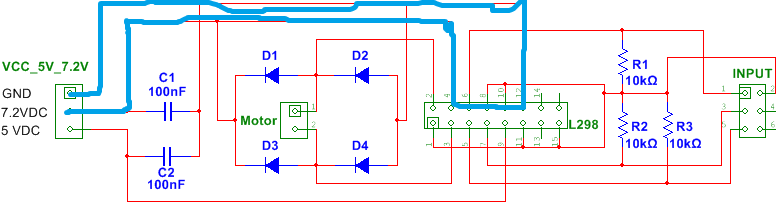
\includegraphics[width=\textwidth]{../fig/billeder/hbro_multisim_loop.png}
\caption{Design af motorens Hbro i Multisim.}
\label{fig:hbro_multisim}
\end{figure}

Pga. problemerne er printet til motorkredsløbet forsøgt designet således, at de strømloops der er, konstrueres så små som mulige og at banerne med stor risiko for støj er placeret så langt som muligt fra andre baner. Desuden er der placeret et Ground plan, der reducerer støj yderligere som et AC-dødt mellemled. Printudlægget kan ses på figur \ref{fig:hbro_ultiboard}.
Som en ekstra forsikring mod common-modestøj, kan man med tilledningerne ud til motoren påsætte en magnet omkring, som derved vil fjerne meget af støjen fra den strøm som løber ud til motoren.

\begin{figure}[h]
\centering
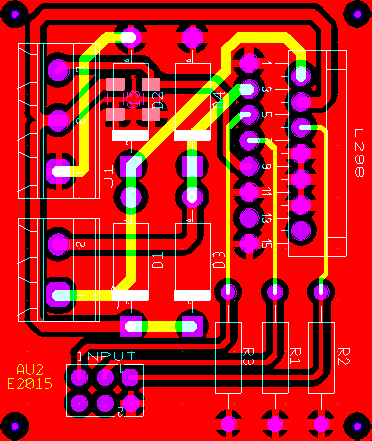
\includegraphics[scale=1]{../fig/billeder/hbro_ultiboard.png}
\caption{Printdesign af motorens Hbro i Ultiboard.}
\label{fig:hbro_ultiboard}
\end{figure}

